\section{Laboratory}
\label{sec:op.laboratory}

This chapter is introductory and does not present any optimization algorithms, but it does introduce two very important concepts: the derivative and the gradient. The goals of this chapter are to become familiar with Python and numpy, learn how to write the pseudocode of the algorithms, and then convert it to Python.

\subsection{Environment}

Make sure you have Python installed. If you don't, follow the tutorial on the official site\footnote{\url{https://www.python.org/}}.

To make sure you have all the libraries installed, run:
\begin{adjustwidth}{1cm}{}
    \texttt{pip install numpy, matplotlib}
\end{adjustwidth}

I recommend that you create a folder where you put all the lab files. To test how everything works, let's create a file called \texttt{test.py} and write into it:

\begin{python}
import matplotlib as mpl
import matplotlib.pyplot as plt
import numpy as np

def f(x):
    return np.cos(x[0], 2) + np.pow(x[1], 2) - 1.5 * x[0] * x[1]

def visualize(f):
    x = np.linspace(-10, 10, 100)
    y = np.linspace(-10, 10, 100)
    X,Y = np.meshgrid(x, y)
    Z = f([X, Y])

    fig = plt.figure(figsize=(14,6))

    ax = fig.add_subplot(1, 2, 1, projection='3d')
    ax.plot_surface(X, Y, Z, rstride=4, cstride=4, linewidth=0, alpha=.8)

    plt.show()

def main():
    visualize(f)

if __name__ == '__main__':
    main()
\end{python}

Run the file and if the following window appears, everything is working correctly!
\begin{center}
    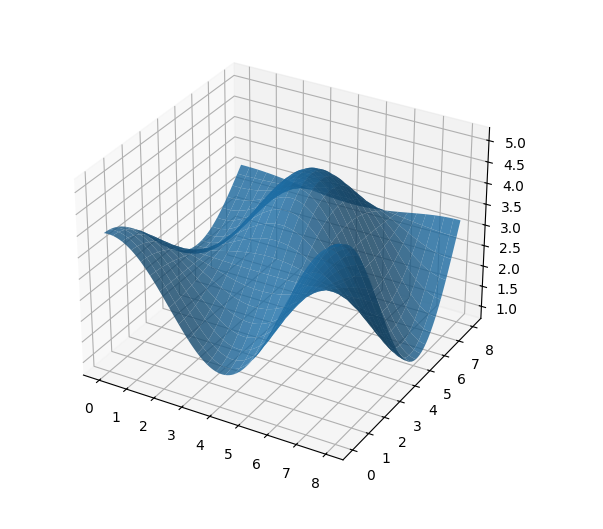
\includegraphics[width=0.7\textwidth]{content/optimization_problems/img/test.png}
\end{center}


\subsection{Exercise: derivative}

Write the pseudocode that calculates the derivative. The function must have three parameters: a function, a point \( x \), and a value of \( h \). \( h \) is optional and if not set takes the value of \( 0.01 \).

\SetKwProg{Fn}{Function}{:}{}
\DontPrintSemicolon    

A possible solution is:
\begin{algorithm}
    \Fn{derivative(f, x, \( h \leftarrow 0.01 \))}{
        \( \mathit{fx} \leftarrow f(x) \)\;
        \( \mathit{fdx} \leftarrow f(x + h) \)\;
        \KwRet \( (\mathit{fdx} - \mathit{fx}) / h \)\;
    }
\end{algorithm}

Now, implement the function in Python. Create a file called \texttt{lab1.py}, then copy and complete the following function:
\begin{python}
import numpy as np

def derivative(f, x, h=0.01):
    # code
    return ...
\end{python}

Add a main function where you create a function, select a point, and call the derivative function to test if it works.
\begin{python}
def main():
    def f(x):
        return x**2 + 2*x + 5
    
    der = derivative(f, 3)
    print("The result is {}".format(der))
\end{python}

Finally, we need to invoke the main function when the program is executed.
\begin{python}
if __name__ == '__main__':
    main()
\end{python}

The result should be:
\begin{python}
import numpy as np

def derivative(f, x, h=0.01):
    # code
    return ...

def main():
    def f(x):
        return x**2 + 2*x + 5
    
    der = derivative(f, 3)
    print("The result is {}".format(der))

if __name__ == '__main__':
    main()
\end{python}

The output sould be:
\begin{adjustwidth}{1cm}{}
    \texttt{The result is 8.009999999999806}
\end{adjustwidth}


\subsection{Excercise: gradient}

Write the pseudocode to compute the gradient in any number of dimensions, the function template is:
\begin{algorithm}
    \Fn{gradient(\( f, x = (x_1, ..., x_n), h \leftarrow 0.01 \))}{
        \tcp{code}
        \KwRet ... \;
    }
\end{algorithm}

Then add a function named \textit{gradient} to \texttt{lab1.py} with the following structure:
\begin{python}
def gradient(f, x, h=0.01):
    # code
    return ...
\end{python}

and modify the main function to add:
\begin{python}
def main():
    # previous code

    def f2(x):
        return np.cos(0.8 * x[0]) * np.cos(0.6 * x[1]) * np.exp(0.1 * x[0]) + 3

    x = [1, 4]
    grad = gradient(f2, x)
    print("The gradient of f2 in (1, 4) is ({}, {})".format(grad[0], grad[1]))
\end{python}

The output should be:
\begin{adjustwidth}{1cm}{}
    \texttt{The gradient of f2 in (1, 4) is (0.41316061821610184, -0.3110320108611564)}
\end{adjustwidth}
